% Project Homepage: https://www.media.mit.edu/groups/open-agriculture-openag/overview/
% Design Repositories: https://github.com/OpenAgricultureFoundation
% PFC White Paper: PDF in Discord
    % Citation: \cite{mit-openag}
% OpenAG White Paper: PDF in Discord
    % Citation: \cite{mit-pfc}

% Half-decent summary: https://www.notion.so/Open-Agriculture-Initiative-OpenAG-cfa5031e2b244093a37158fe1a99ec12

% Introduction

The Open Agriculture Initiative (OpenAG) is a project launched by the MIT Media Lab with the goal to "Build open resources to enable a global community to accelerate digital agricultural innovation." 

One of their primary developments was an open-source controlled-environment agriculture micro-greenhouse, the Personal Food Computer.
The PFC controls all environmental growing parameters and collects data during the growth cycle.
Data can be collected by users and shared between members of the open-source community.
This allows for the creation of reproducible "climate recipes" where other devices with similar abilities can reliably generate the same environment and attain the same plant growth results.

% Graphics

\begin{figure}[h]
    \centering
    \begin{subfigure}[b]{0.08\textwidth}
        \hfill
    \end{subfigure}
    \begin{subfigure}[b]{0.40\textwidth}
        \centering
        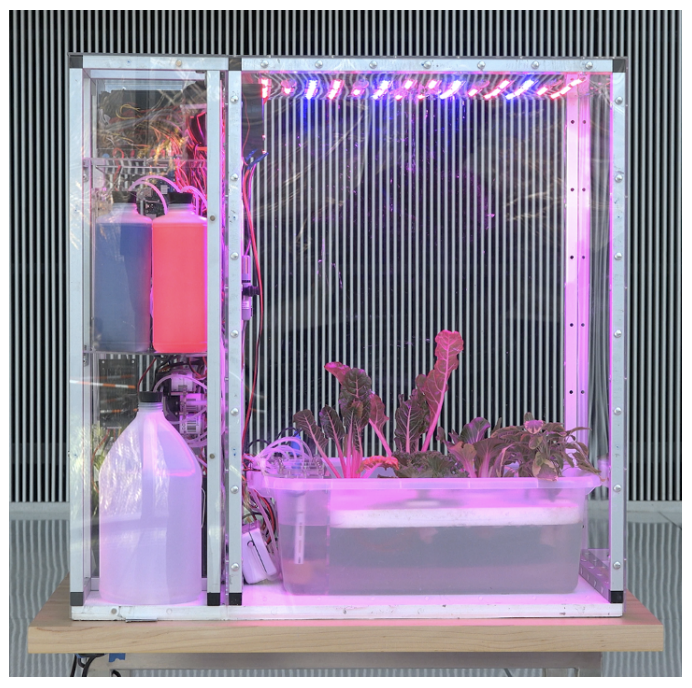
\includegraphics[width=\textwidth]{../assets/pfc-built.png}
        \caption{Assembled PFC v1.}
        \label{fig:pfc-built}
    \end{subfigure}
    \hfill
    \begin{subfigure}[b]{0.26\textwidth}
        \centering
        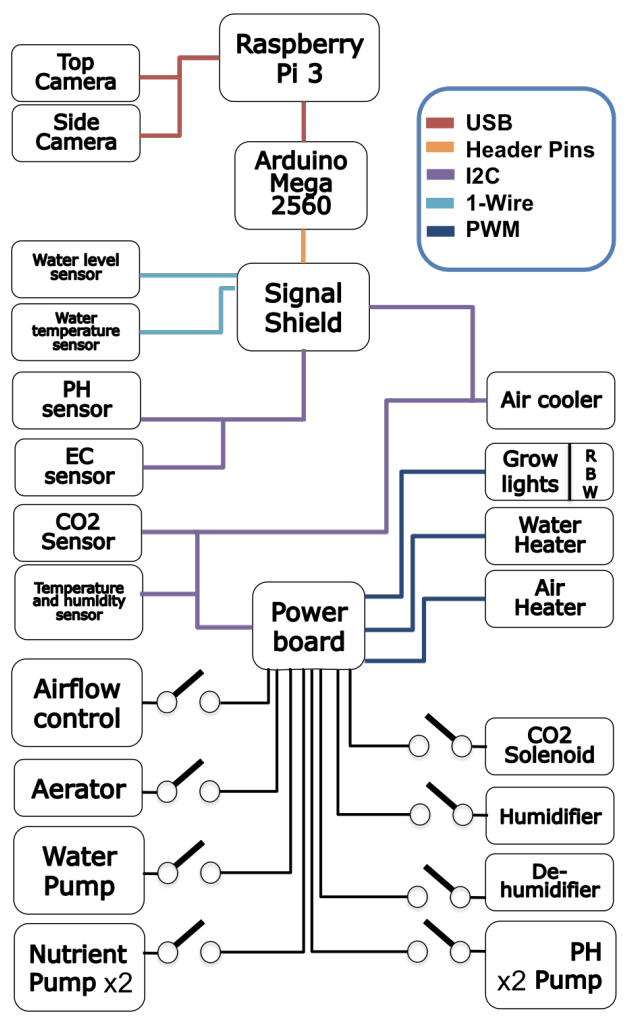
\includegraphics[width=\textwidth]{../assets/pfc-components.png}
        \caption{Component diagram.}
        \label{fig:pfc-components}
    \end{subfigure}
    \begin{subfigure}[b]{0.10\textwidth}
        \hfill
    \end{subfigure}
    \caption{From \cite{mit-pfc}.}
    \label{fig:pfc}
\end{figure}

One of the design's major flaws is in its implementation. Despite the claim that the PFC focusses on \ref{sc:3} and \ref{sc:5}, in practice, it failed to meet \ref{r:3} \cite{mit-basil}.
In addition, the PFC utilizes Deep Water Culture (DWC) hydroponics \cite{mit-pfc}, as opposed to aeroponics, resulting in a lowered water efficiency.

The PFC is also much more focussed on \ref{sc:3} and \ref{sc:5} than \ref{r:1} and \ref{r:1a}, meaning that they valued optimization and data collection over bulk yield of food outputs. This shows in that their design did not account for scalability of output \cite{mit-wfp}.

However, the array of sensors included in the design (both plant-growth and environmental) as well as the principle of plant phenomenology optimization is informative in meeting \ref{r:3} and their attempts can serve as a basis for understanding \ref{sc:3} and \ref{sc:5} \cite{mit-openag}.

\textbf{Attempted}: \ref{ll:output_variety}, \ref{ll:output_palatability} (via \ref{sc:5}), \ref{ll:control_airtemp}. \ref{ll:control_airhum}, \ref{ll:control_light}, \ref{ll:control_aircirculation}, \ref{ll:control_nutrientsolution}, \ref{ll:automation}

\textbf{Did Not Consider}: \ref{ll:output_energy}, \ref{ll:insulateisolate}, \ref{ll:germinationsuccess}, \ref{ll:efficiency_energy}, \ref{ll:efficiency_water}, \ref{ll:time_germination}, \ref{ll:time_growth}, \ref{ll:time_harvest}, \ref{ll:crosscontamination}
